\documentclass{article}

\usepackage{mathtools,amsfonts}
\usepackage{enumerate}
\usepackage{fancyvrb}
\usepackage{graphicx}


\begin{document}
	\thispagestyle{empty}
	
	\begin{center}
		\textbf{\Large Intermediate Test 3}
		% LEVEL is Senior, Intermediate or Beginner
		% NUMBER is the test number: 1, 2, etc.
		\\ \vspace{1em}
		\textbf{\large Stellenbosch Camp 2019}
		\\ \vspace{1em}
		\textbf{\large Time: $2\frac{1}{2}$ hours}
	\end{center}
	
	\vspace{6.81mm}
	
	\begin{enumerate}[1.]
		\item % Emile, C
		Find the number of paths from $A$ to $B$ where the only allowed moves are moving down along a diagonal line or moving left or right along a horizontal line, but never crossing the same line twice.
		
		\begin{center}
			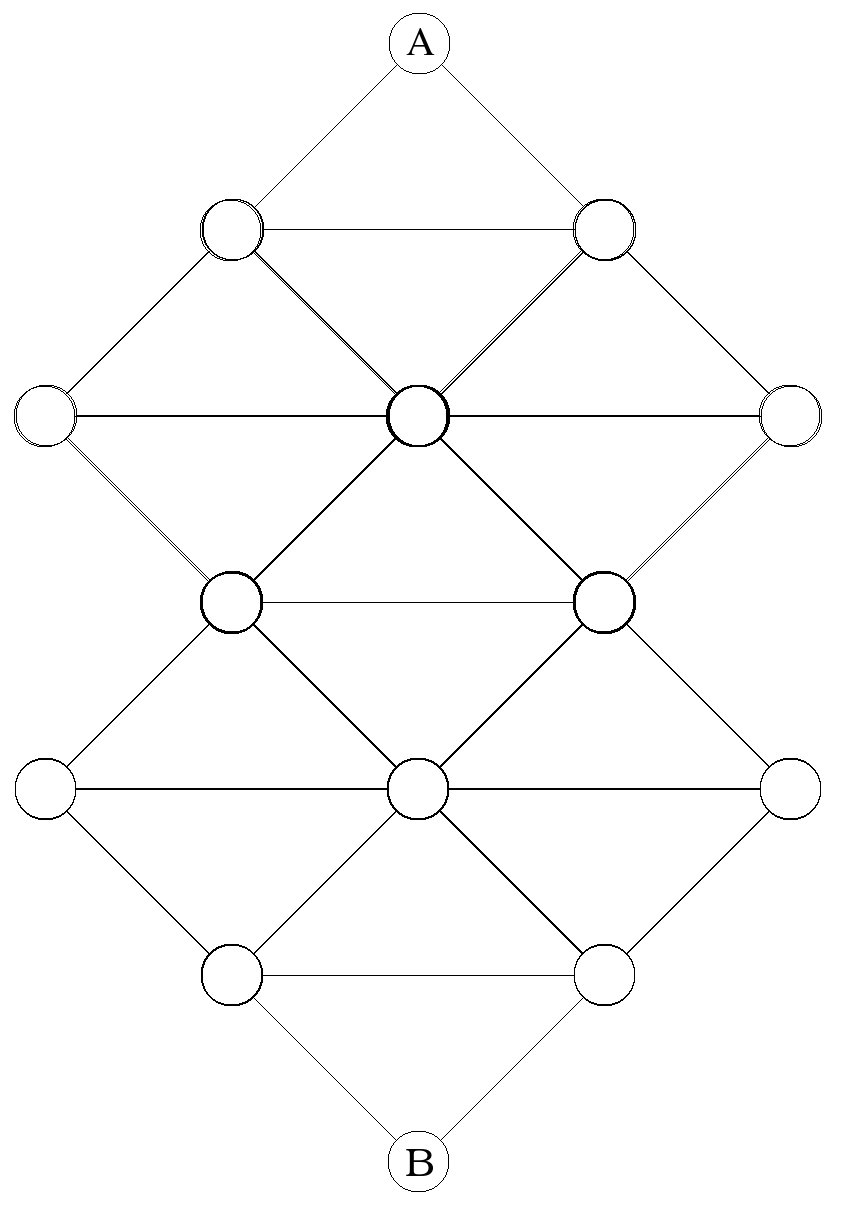
\includegraphics[width=0.35\textwidth]{test_3_q_1}
		\end{center}
		\vspace{6.81mm}

		\item % PAMO 2016 Q1, G 
		Two intersecting circles, $C_1$ and $C_2$, have a common tangent which touches $C_1$ at $P$ and $C_2$ at $Q$. The two circles intersect at $M$ and $N$, where $N$ is nearer to $PQ$ than $M$ is. The line $PM$ meets the circle $C_2$ again at $R$. Prove that $MQ$ bisects $\angle PMR$.
		\vspace{6.81mm}

		\item % Emile, C
		Emma and Emile play a game on a $2019 \times 2019$ board made up of unit grid squares. Emma plays first by placing a knight on one of the squares and thereafter they take turns to place a knight on a square that does not already contain a knight and is not attacked by one of the already placed knights. The first player who cannot do this loses. Can one of the players always guarantee that they will win? If so, which one? 
		\vspace{6.81mm}
		
		\item % Moldova 2018 8.6, A
		Let $a$, $b$, and $c$ be positive real numbers such that $b, c \in [1,2)$ and
		\[ \frac{a+b}{b(1+c)} +\frac{a+c}{c(1+b)} = 2. \]
		Show that $a$, $b$, and $c$ are the lengths of the sides of a triangle.
		\vspace{6.81mm}

		\item % The Phil, N
		Find the least positive integer $k$ such that $2050^{2051}$ can be written as a sum of $k$ $5$th powers.

			
	\end{enumerate}
	
	
\vfill
% ASCII art
\begin{center}
\begin{BVerbatim}

                  /^----^\
                  | 0  0 |
                  |  \/  |
                 /       \
                |     |;;;|
                |     |;;;|          \   \
                |      \;;|           \\//
                \       \|           / /
------------------(((--(((------------\ \----------,
--  ___  ----  __ ---   ____   ---- _____ -- __ - \
__ --   __ -- _____ --- __  ----  ___  ---- __ -- /
---------------/ /---------------\  \--------------`
               \ \               / /
                //\             //
                \               \\
                                /

\end{BVerbatim}
\end{center}
	
\end{document}
